%
% graphisch.tex
%
% (c) 2020 Prof Dr Andreas Müller, Hochschule Rapperswil
%
\begin{figure}
\centering
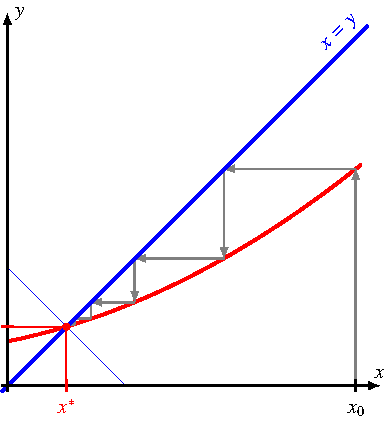
\includegraphics{chapters/10-arithmetik/figures/normal.pdf}
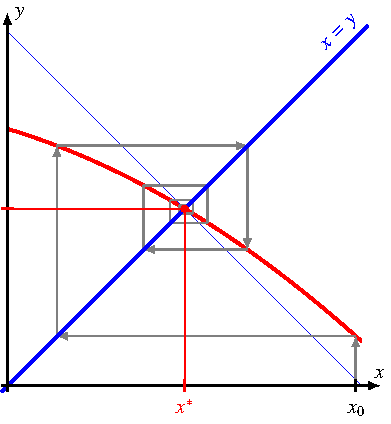
\includegraphics{chapters/10-arithmetik/figures/negativ.pdf}
\caption{Die Fixpunktiteration $x_{n+1}=f(x_n)$ konvergiert gegen
den Fixpunkt $x^*$ falls $|f'(x^*)|<1$ mit
mindestens linearer Konvergenzgeschwindigkeit.
\label{buch:figure:fixpunkt:normal}}
\end{figure}
%
\begin{figure}
\centering
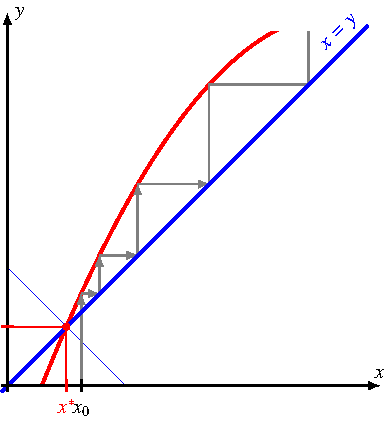
\includegraphics{chapters/10-arithmetik/figures/divergent.pdf}
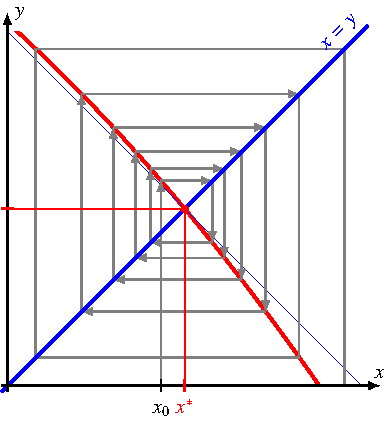
\includegraphics{chapters/10-arithmetik/figures/negdiv.pdf}
\caption{Die Fixpunktiteration $x_{n+1}=f(x_n)$ mit Fixpunkt $x^*$
divergiert für $|f'(x^*)|>1$.
\label{buch:figure:fixpunkt:divergent}}
\end{figure}
%
\begin{figure}
\centering
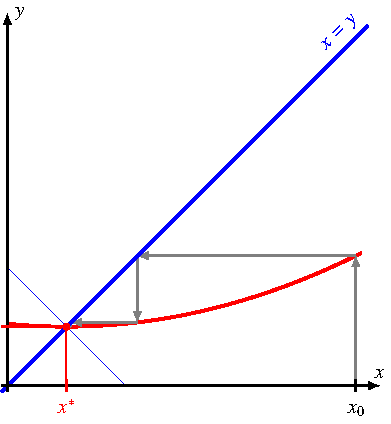
\includegraphics{chapters/10-arithmetik/figures/quadratisch.pdf}
\caption{Die Fixpunktiteration $x_{n+1}=f(x_n)$ konvergiert quadratisch
gegen den Fixpunkt $x^*$
für $f'(x^*)=0$.
\label{buch:figure:fixpunkt:quadratisch}}
\end{figure}
%
\begin{figure}
\centering
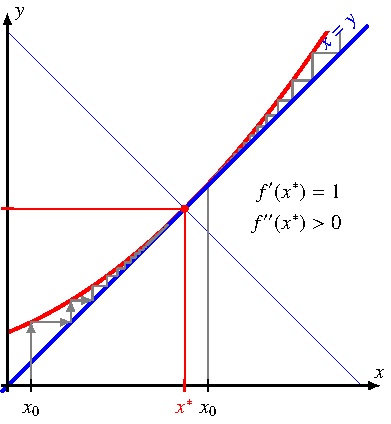
\includegraphics{chapters/10-arithmetik/figures/m1qp.pdf}
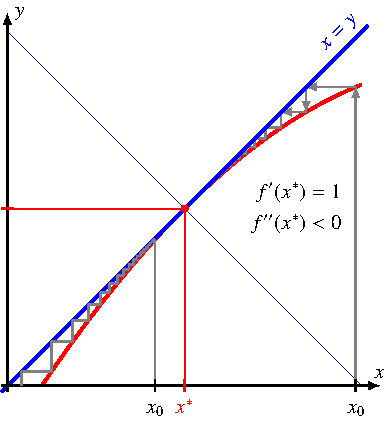
\includegraphics{chapters/10-arithmetik/figures/m1qn.pdf}
\caption{Konvergenzverhalten der Fixpunktiteration $x_{n+1}=f(x_n)$
in der Umgebung des Fixpunktes $x^*$ für $f'(x^*)=1$.
Falls $f''(x^*)>0$ konvergiert die Iteration sehr langsam
für einen Startwert $x_0>x^*$ falls $f''(x^*)>0$, divergiert
aber für einen Startwert $x_0>x^*$. 
Bei negativer zweiter Ableitung ist es umgekehrt.
\label{buch:figure:fixpunkt:abl1}}
\end{figure}
\begin{figure}
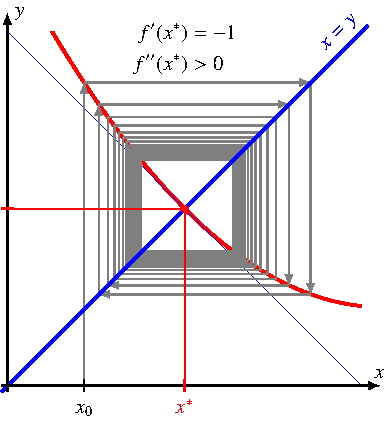
\includegraphics{chapters/10-arithmetik/figures/mnqp.pdf}
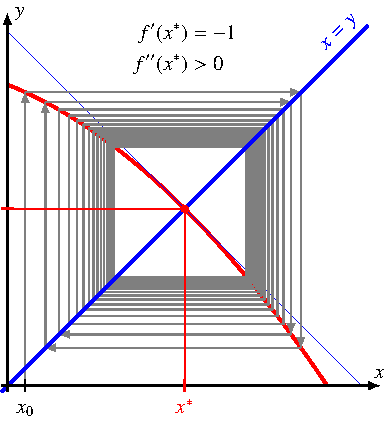
\includegraphics{chapters/10-arithmetik/figures/mnqn.pdf}
\caption{Die Fixpunktiteration $x_{n+1}=f(x_n)$ konvergiert sehr langsam
in der Umgebung des Fixpunktes $x^*$ für
$f'(x^*)=-1$ für $f''(x^*)\ne 0$.
\label{buch:figure:fixpunkt:ablm1}}
\end{figure}
%
%\begin{figure}
%\centering
%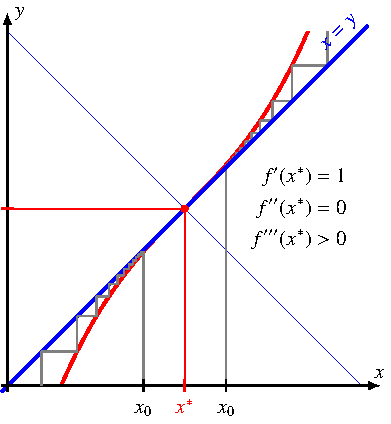
\includegraphics{chapters/10-arithmetik/figures/m1kp.pdf}
%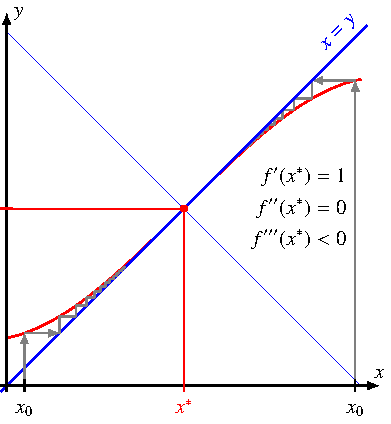
\includegraphics{chapters/10-arithmetik/figures/m1kn.pdf}
%\caption{Die Fixpunktiteration $x_{n+1}=f(x_n)$ mit Fixpunkt $x^*$
%mit $f'(x^*)=1$ und $f''(x^*)=0$ divergiert für $f'''(x^*)>0$
%und konvergiert sehr langsam für $f'''(x^*)<0$.
%\label{buch:figure:fixpunkt:abl1kub}}
%\end{figure}
%%
%\begin{figure}
%\centering
%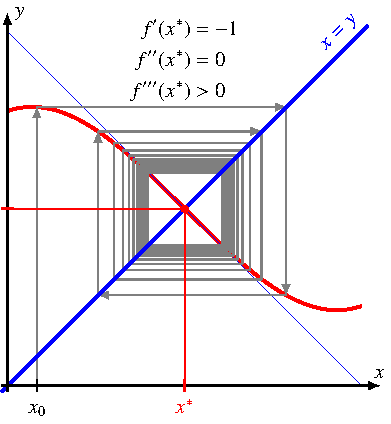
\includegraphics{chapters/10-arithmetik/figures/mnkp.pdf}
%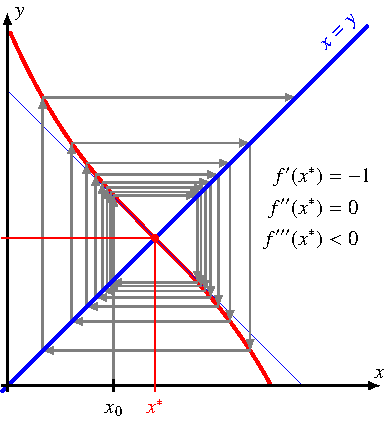
\includegraphics{chapters/10-arithmetik/figures/mnkn.pdf}
%\caption{Die Fixpunktiteration $x_{n+1}=f(x_n)$ mit Fixpunkt $x^*$
%mit $f'(x^*)=-1$ und $f''(x^*)=0$ konvergiert sehr langsam für $f'''(x^*)>0$
%und divergiert für $f'''(x^*)<0$.
%\label{buch:figure:fixpunkt:ablm1kub}}
%\end{figure}
